% ==============================================================================
% Seminar Talk: Inside Synthetic Dollar Liquidity and the
%               Microstructure of FX Swap Markets
% Format: Beamer, 25–35 slides, Theory+Empirics arc
% Audience: Applied finance/economics seminar (PhD students + faculty)
% ==============================================================================

\documentclass[aspectratio=169, 10pt]{beamer}

% ====== Core Packages ======
\usepackage{amsmath, amssymb, amsfonts, mathtools, dsfont}
\usepackage{booktabs}
\usepackage{graphicx}
\usepackage{tikz}
\usepackage{xcolor}
\usepackage{hyperref}
\usepackage[nameinlink]{cleveref}

% ====== Theme ======
\usetheme{Madrid}
\usecolortheme{default}
\setbeamertemplate{footline}[frame number]
\setbeamertemplate{navigation symbols}{}
\setbeamertemplate{itemize items}[circle]
\setbeamertemplate{enumerate items}[default]

% ====== Colors ======
\definecolor{accent}{RGB}{0, 127, 255}
\definecolor{resultcol}{RGB}{0, 127, 255}
\definecolor{dimgray}{RGB}{120, 120, 120}

% ====== Notation Commands ======
\newcommand{\calB}{\mathcal{B}}      % aggregate demand slope
\newcommand{\mustar}{\mu_t^{*}}      % equilibrium spread
\newcommand{\thetaT}{\theta_t}       % market tightness
\newcommand{\Bt}{B_t}                % intermediary capacity
\newcommand{\Ut}{U_t}                % seeker mass
\newcommand{\Mt}{M_t}                % matches
\DeclareMathOperator*{\argmax}{arg\,max}

% ====== Helper: highlighted result box ======
\newcommand{\resultbox}[1]{%
  \begin{center}
    {\large\color{resultcol}\textbf{#1}}
  \end{center}}

% ====== Title Info ======
\title[FX Swap Microstructure]{Inside Synthetic Dollar Liquidity\\
  and the Microstructure of FX Swap Markets}
\subtitle{}
\author[Author]{[Author Name]}
\institute[Institution]{[University / Institution]}
\date{\today}

% ==============================================================================
\begin{document}
% ==============================================================================

% ------------------------------------------------------------------------------
% TITLE SLIDE
% ------------------------------------------------------------------------------
\begin{frame}
  \titlepage
\end{frame}

% ------------------------------------------------------------------------------
\section{Motivation}
% ------------------------------------------------------------------------------

% SLIDE 1 — Hook: March 2020
\begin{frame}{March 2020: The Dollar Plumbing Failed}

  \begin{columns}
    \begin{column}{0.48\textwidth}
      \textbf{What happened:}
      \begin{itemize}
        \item Foreign banks scrambled for dollar funding
        \item The cross-currency basis \emph{spiked} to its largest level since the GFC
        \item The Fed deployed \$450 billion in swap lines within days
      \end{itemize}

      \bigskip

      \textbf{The puzzle:}\\
      Dollars were abundant inside the Federal Reserve system.\\[0.5em]
      Yet foreign banks \emph{could not obtain them} at normal prices.
    \end{column}
    \begin{column}{0.50\textwidth}
      \begin{center}
        % Figure: tightness and premium time series — reference actual file
        \includegraphics[width=\textwidth]{../figures/tightness_premium_ts.pdf}\\
        {\scriptsize\color{dimgray}
          Market tightness $\thetaT$ (top) and funding premium $\mu_t$ (bottom).
          Vertical dashed line: March 2020. Shaded: quarter-end months.
          Source: synthetic regulatory bilateral FX swap data.}
      \end{center}
    \end{column}
  \end{columns}

  \note{
    Open with the March 2020 episode — the most vivid demonstration of the inside/outside
    distinction in recent memory. The key message: dollar shortage was not about dollar scarcity
    in aggregate, but about the failure of the conversion mechanism.
    Point to the spike in the right panel. Quarter-end patterns visible too — foreshadow Prop 4.
    Anticipated question: ``Is this just a risk-off story?'' -- Answer: time FE absorb aggregate risk;
    our instrument identifies cross-market differential demand. Backup: robustness slide.
  }
\end{frame}

% SLIDE 2 — Inside vs. Outside Dollar Liquidity
\begin{frame}{Two Kinds of Dollar Liquidity}

  \begin{columns}
    \begin{column}{0.48\textwidth}
      \textbf{Outside safe dollars} $O_t$
      \begin{itemize}
        \item Federal Reserve reserve balances
        \item US Treasuries, FDIC-insured deposits
        \item Central-bank swap lines
      \end{itemize}
      \medskip
      {\color{dimgray} Backstopped by the US monetary core.}
    \end{column}
    \begin{column}{0.48\textwidth}
      \textbf{Inside synthetic dollars} $I_t$
      \begin{itemize}
        \item FX swaps, offshore repo
        \item Eurodollar deposits
        \item Wholesale global bank funding
      \end{itemize}
      \medskip
      {\color{dimgray} Produced \emph{outside} the US domestic banking system.}
    \end{column}
  \end{columns}

  \bigskip\bigskip

  \begin{center}
    \textbf{In normal times:} near-perfect substitutes. Arbitrage $\Rightarrow$ basis $\approx 0$.\\[0.5em]
    \textbf{In stress:} \emph{not} substitutes. Converting $I_t \to O_t$ requires finding\\
    a counterparty. That search can fail.
  \end{center}

  \note{
    This slide introduces the inside/outside distinction — the conceptual core of the paper.
    Stress the point that March 2020 was a run FROM inside TO outside dollars, not a run on
    the dollar itself.
    Anticipated question: ``How is this different from the CIP literature?''
    Answer: CIP measures price. We model the matching process that determines that price.
    No backup slide needed -- this is conceptual setup.
  }
\end{frame}

% SLIDE 3 — The Question
\begin{frame}{The Question}

  \bigskip

  \resultbox{What determines the premium on inside synthetic dollar liquidity?}

  \bigskip\bigskip

  \textbf{Three forces in equilibrium:}

  \medskip

  \begin{tabular}{clp{6.5cm}}
    \toprule
    Symbol & Force & Role \\
    \midrule
    $\Ut$ & Demand (seeker mass) & Foreign banks seeking synthetic dollars \\
    $\Bt$ & Supply capacity & Dealer / FBO balance-sheet capacity \\
    $\thetaT = \Ut/\Bt$ & Market tightness & The price-relevant ratio \\
    \bottomrule
  \end{tabular}

  \bigskip

  \textbf{Approach:} Model a matching market $\to$ derive comparative statics $\to$ test with IV.

  \note{
    One slide, one idea: the premium is determined by the tightness ratio theta.
    This slide bridges motivation and model. Point out that theta is the sufficient statistic.
    Anticipated question: ``Why matching? Why not price discovery / information models?''
    Answer: FX swaps are bilateral OTC markets with genuine search frictions -- dealers
    don't post quotes; relationships and rolodexes matter.
  }
\end{frame}

% ------------------------------------------------------------------------------
\section{Model}
% ------------------------------------------------------------------------------

% SLIDE 4 — The Environment
\begin{frame}{Environment: A Matching Market for Dollar Conversion}

  \textbf{Actors:}
  \begin{itemize}
    \item \textbf{Foreign banks} (FBO) --- dollar \emph{seekers}: need dollars, have foreign currency
    \item \textbf{Primary dealers / US banks} --- dollar \emph{suppliers}: convert at a price
    \item \textbf{Hedge funds} --- opportunistic suppliers when the basis exceeds entry cost
    \item \textbf{Central banks} --- counter-cyclical suppliers via swap lines
  \end{itemize}

  \bigskip

  \textbf{What happens in each period:}
  \begin{enumerate}
    \item $\Ut$ seekers and $\Bt$ suppliers meet via the matching technology
    \item Matching probability $p_t$ determines conversion quality $\chi_t \in (0,1]$
    \item Market-clearing spread $\mustar$ equates aggregate net demand to zero
  \end{enumerate}

  \note{
    This is the environment slide -- set the stage before showing the matching function.
    Emphasize the search friction: not every seeker finds a counterparty.
    Anticipated question: ``Why don't seekers post higher prices to attract more suppliers?''
    Answer: that's exactly what the equilibrium spread does -- mu* is the price that clears the market.
  }
\end{frame}

% SLIDE 5 — Matching Function (build up with pause)
\begin{frame}{The Matching Technology}

  Total matches between seekers and suppliers:
  \[
    \Mt = \eta\, \Ut^{\gamma}\, \Bt^{1-\gamma}
  \]
  \pause

  \textbf{Matching probability for a seeker:}
  \[
    p_t = \frac{\Mt}{\Ut} = \eta \left(\frac{\Bt}{\Ut}\right)^{1-\gamma}
        = \eta\,\thetaT^{-(1-\gamma)}
  \]
  \pause

  \textbf{Key property:} $p_t$ is strictly \emph{decreasing} in tightness $\thetaT = \Ut/\Bt$.

  \bigskip
  \begin{columns}
    \begin{column}{0.55\textwidth}
      \begin{itemize}
        \item $\Ut \uparrow$ $\Rightarrow$ $\thetaT \uparrow$ $\Rightarrow$ $p_t \downarrow$ $\Rightarrow$ quality $\chi_t \downarrow$
        \item $\Bt \uparrow$ $\Rightarrow$ $\thetaT \downarrow$ $\Rightarrow$ $p_t \uparrow$ $\Rightarrow$ quality $\chi_t \uparrow$
      \end{itemize}
    \end{column}
    \begin{column}{0.42\textwidth}
      {\color{dimgray}\small
        $\eta > 0$: matching efficiency\\
        $\gamma \in (0,1)$: demand-side elasticity}
    \end{column}
  \end{columns}

  \note{
    Build with pauses. First show the matching function. Then the per-seeker probability.
    Then the key monotonicity property.
    This slide is the mechanism. Everything else follows from: more seekers per supplier
    means worse matching, which degrades quality, which raises the required spread.
    Anticipated question: ``Why Cobb-Douglas?'' -- tractability and CRS. Lemma 1 in the paper
    proves the key properties hold under this functional form.
  }
\end{frame}

% SLIDE 6 — Equilibrium Spread
\begin{frame}{Equilibrium: The Price Function}

  Each sector $s$ chooses a signed net USD position linear in the spread:
  \[
    \mathfrak{q}_{s,m,t} = \alpha_{s,m} + \beta_s\,\mu_{m,t} + \gamma_s X_{s,m,t} + \varepsilon_{s,m,t}
  \]

  \bigskip

  Market clearing ($\sum_s \mathfrak{q}_{s,m,t} = 0$) under $\calB \equiv \sum_s \beta_s < 0$:

  \[
    \boxed{\mustar = -\frac{1}{\calB} \sum_s \bigl[\alpha_{s,m} + \gamma_s X_{s,m,t} + \varepsilon_{s,m,t}\bigr]}
  \]

  \bigskip

  \begin{columns}
    \begin{column}{0.55\textwidth}
      \textbf{Intuition:}
      \begin{itemize}
        \item $\calB < 0$: aggregate demand is downward-sloping
        \item Spread rises when aggregate demand shifts up (tightness $\uparrow$)
        \item $|\calB|$ small $\Rightarrow$ large price impact per unit demand shock
      \end{itemize}
    \end{column}
    \begin{column}{0.42\textwidth}
      {\color{dimgray}\small
        \textbf{Maintained hypothesis:} $\calB < 0$\\
        Tested ex post via demand system\\
        (Section~5 / Structural Extension)}
    \end{column}
  \end{columns}

  \note{
    This is the price equation. The maintained hypothesis B < 0 is testable -- we verify it
    in the demand system. Theorem 1 in the paper proves existence and uniqueness.
    Anticipated question: ``What if B > 0?'' -- Then the equilibrium pricing equation fails.
    The demand system estimate (B_hat < 0, significant) confirms the maintained hypothesis.
    Backup: demand system results slide.
  }
\end{frame}

% SLIDE 7 — Proposition 1: Demand
\begin{frame}{Proposition 1: Demand Pressure Raises the Premium}

  \begin{block}{Proposition 1}
    At any interior equilibrium, $\partial \mustar / \partial \Ut > 0$:\\
    an increase in the mass of seekers raises the equilibrium funding spread,\\
    holding intermediary capacity $\Bt$ fixed.
  \end{block}

  \bigskip

  \textbf{Mechanism} (chain rule through quality):
  \[
    \frac{\partial \mustar}{\partial \Ut}
    = \underbrace{\frac{\partial \mustar}{\partial \chi_t}}_{<\,0}
    \cdot \underbrace{\chi'(p_t)}_{>\,0}
    \cdot \underbrace{\frac{\partial p_t}{\partial \Ut}}_{<\,0}
    \;>\; 0
  \]

  \bigskip

  \textbf{Testable prediction:} the IV estimate $\hat\beta \to -\gamma_{FB}/\calB > 0$\\
  {\color{dimgray}\small where $\gamma_{FB}$ is the foreign-bank demand loading on the MMF shock.}

  \note{
    One proposition per slide. Show the chain of signs clearly.
    This is the primary empirical target. The IV design (next section) is designed
    to identify exactly this derivative.
    Anticipated question: ``Can supply respond to demand shocks and mute the effect?''
    Answer: Yes, and this attenuates OLS. The IV corrects for it -- IV > OLS is consistent
    with supply-side accommodation attenuating the raw price response.
  }
\end{frame}

% SLIDE 8 — Proposition 2: Capacity
\begin{frame}{Proposition 2: Capacity Tightening Amplifies Price Impact}

  \begin{block}{Proposition 2}
    $\partial \mustar / \partial \Bt < 0$: higher capacity lowers the premium.\\[0.3em]
    Moreover, the price impact of demand shocks is \emph{larger} when capacity is low:
    \[
      \left.\frac{\partial \mustar}{\partial \Ut}\right|_{B_t = B^{\text{low}}}
      \;>\;
      \left.\frac{\partial \mustar}{\partial \Ut}\right|_{B_t = B^{\text{high}}}
    \]
  \end{block}

  \bigskip

  \textbf{The amplification result:}
  $\bigl|\partial p_t / \partial \Ut\bigr| = \eta(1-\gamma)\thetaT^{-(2-\gamma)} / \Bt$
  is larger when $\Bt$ is smaller.

  \bigskip
  Same demand shock $\Rightarrow$ larger $\Delta\thetaT$ $\Rightarrow$ larger premium response
  when dealer capacity is already thin.

  \note{
    The amplification prediction motivates the DealerConstraint interaction in the empirics.
    Stress: we can't cleanly ID the causal effect of B_t (constraints tighten in stress),
    so the empirical test is stated as effect heterogeneity across capacity regimes.
    Anticipated question: ``How is DealerConstraint defined?''
    Answer: indicator for when primary dealer repo borrowings fall below the 25th percentile
    of their rolling 4-quarter distribution. Details in Table 3 notes (backup).
  }
\end{frame}

% SLIDE 9 — Proposition 3: Convexity (theory-only)
\begin{frame}{Proposition 3: Non-linearity and Threshold Effects}

  \begin{block}{Proposition 3}
    Under additional regularity on quality ($\chi'' > 0$) and the price function
    ($\Phi'' > 0$):
    \[
      \frac{\partial^2 \mustar}{\partial \thetaT^2} > 0
    \]
    There exists a threshold $\theta^* > 0$ above which the rate of increase
    $\partial \mustar / \partial \thetaT$ escalates sharply.
  \end{block}

  \bigskip

  \begin{columns}
    \begin{column}{0.50\textwidth}
      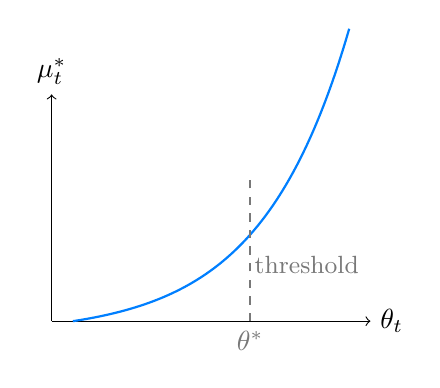
\begin{tikzpicture}[scale=0.9]
        \draw[->] (0,0) -- (4.5,0) node[right] {$\thetaT$};
        \draw[->] (0,0) -- (0,3.2) node[above] {$\mustar$};
        \draw[thick, accent, domain=0.3:4.2, samples=80]
          plot (\x, {0.15*exp(0.8*\x) - 0.15*exp(0.8*0.3)});
        \draw[dashed, dimgray] (2.8,0) node[below] {$\theta^*$} -- (2.8,2);
        \node[dimgray, align=left, font=\small] at (3.6,0.8) {threshold};
      \end{tikzpicture}
    \end{column}
    \begin{column}{0.47\textwidth}
      {\color{dimgray}\small
        \textbf{This is a theoretical result.}\\[0.5em]
        Direct testing requires a threshold specification beyond current scope.\\[0.5em]
        Motivates: focus on March 2020 and quarter-end episodes as high-$\thetaT$ regimes.}
    \end{column}
  \end{columns}

  \note{
    Critical: this is THEORETICAL ONLY. Do not suggest an empirical test.
    The paper explicitly states testing this directly is beyond scope.
    The convex shape is stylized -- drawn from the matching function property
    p''(theta) = eta*(1-gamma)*(2-gamma)*theta^{-(3-gamma)} > 0.
    The slide shows the theoretical shape motivating the crisis/quarter-end focus.
    Anticipated question: ``Could you test this with a threshold regression?''
    Answer: maybe with the confidential data; the synthetic data does not support
    reliable continuous theta measurement (graded C in the feasibility assessment).
  }
\end{frame}

% SLIDE 10 — Proposition 4: Quarter-End
\begin{frame}{Proposition 4: Quarter-End Regulatory Amplification}

  \begin{block}{Proposition 4}
    $\Bt$ contracts deterministically at quarter-end ($Q_t = 1$):\\
    $B_t^{FBO}$ and $B_t^{USbank}$ fall by $\omega > 0$ for regulatory reporting.\\[0.3em]
    By Proposition 2: $\partial^2 \mustar / \partial \Ut \partial Q_t > 0$.
  \end{block}

  \bigskip

  \textbf{Key distinction from Proposition 2:}\\
  \begin{itemize}
    \item Prop.\ 2 (DealerConstraint): endogenous to demand state
    \item Prop.\ 4 (QuarterEnd): \emph{deterministic} timing --- exogenous to concurrent demand
  \end{itemize}

  \bigskip

  {\color{dimgray} Recall: the tightness--premium plot shows clockwork quarter-end spikes
    that dissipate within days.}

  \note{
    Quarter-end is the cleanest test of the capacity channel because the timing is
    regulatory (not stress-driven). The demand-only explanation would require foreign banks
    to spike demand at every quarter-end, which is implausible.
    Anticipated question: ``Couldn't quarter-end demand also be higher?''
    Answer: Yes, but the deterministic timing makes supply the more parsimonious explanation.
    The interaction test cannot distinguish supply vs demand at quarter-end completely --
    we note this limitation explicitly in the paper (Section 4.3).
  }
\end{frame}

% SLIDE 11 — Testable Predictions (bridge to empirics)
\begin{frame}{Testable Predictions: Bridging Model and Data}

  \begin{center}
  \begin{tabular}{clll}
    \toprule
    & Proposition & Prediction & Empirical Test \\
    \midrule
    1 & Demand $\uparrow$ spreads & $\hat\beta > 0$ in IV & Main 2SLS (Table~2) \\
    2 & Capacity $\downarrow$ amplifies & $\hat\beta_2 > 0$ interaction & DealerConstraint $\times$ demand \\
    3 & Convexity / threshold & Theoretical shape & Crisis episodes (descriptive) \\
    4 & Quarter-end spike & $\hat\beta_{QE} > 0$ interaction & QuarterEnd $\times$ demand \\
    \bottomrule
  \end{tabular}
  \end{center}

  \bigskip

  \textbf{Structural bridge:} $\hat\beta \xrightarrow{p} -\gamma_{FB}/\calB$\\
  {\color{dimgray}\small Sign: $\calB < 0$ (tested in demand system). Magnitude: depends on $|\calB|$.}

  \note{
    One clean summary of what the model delivers empirically. Row 3 is theory-only -- no arrow to a test.
    Anticipated question: ``Why can't you test Prop 3 directly?''
    Answer: explained on previous slide -- threshold spec beyond current scope.
    This slide transitions to the data and identification section.
  }
\end{frame}

% ------------------------------------------------------------------------------
\section{Data}
% ------------------------------------------------------------------------------

% SLIDE 12 — Data Structure
\begin{frame}{Data: Bilateral Regulatory Transaction Data}

  \textbf{Cell structure:}
  \[
    \text{cell} = \underbrace{s}_{\text{sector}} \times
                  \underbrace{c}_{\text{country}} \times
                  \underbrace{m}_{\text{pair}} \times
                  \underbrace{k}_{\text{tenor}} \times
                  \underbrace{t}_{\text{date}}
  \]

  \bigskip

  \begin{columns}
    \begin{column}{0.48\textwidth}
      \textbf{What we observe:}
      \begin{itemize}
        \item Both counterparties to each FX swap (name, sector, country)
        \item Taker / maker role --- active demand vs passive supply
        \item Signed USD flow: $> 0$ (demand), $< 0$ (supply)
      \end{itemize}
    \end{column}
    \begin{column}{0.48\textwidth}
      \textbf{Tenor buckets:}\\[0.3em]
      ON, 1W, 1M, 3M, 6M, 1Y+\\[0.5em]
      \textbf{Outcome:}\\[0.3em]
      $\text{PriceUSD}_{m,t} = -\text{TIB}_{m,t}$\\
      {\color{dimgray}(volume-weighted median forward basis)}\\[0.5em]
      $\text{PriceUSD} > 0$ $\Leftrightarrow$ synthetic dollars expensive
    \end{column}
  \end{columns}

  \bigskip

  {\color{dimgray}\small
    Note: paper uses synthetic data constructed to replicate distributional properties
    of confidential regulatory bilateral FX swap transaction data.}

  \note{
    The taker/maker flag is the key data feature -- it lets us separate active demand
    from passive supply, which is central to the matching interpretation.
    Anticipated question: ``How many currency pairs?'' -- Approximately 36 markets
    (pair x tenor combinations). Enough for two-way clustering.
    Anticipated question: ``What's the time series coverage?'' -- 2015--2023 per
    the tightness-premium figure.
  }
\end{frame}

% SLIDE 13 — Intermediation Matrix
\begin{frame}{Who Intermediates Synthetic Dollar Flows?}

  \begin{center}
    \includegraphics[width=0.80\textwidth]{../figures/intermediation_matrix.pdf}\\
    {\scriptsize\color{dimgray}
      Fraction of total dollar supply to the row sector originating from the column sector.
      Averaged over the full sample. Source: synthetic regulatory bilateral FX swap data.}
  \end{center}

  \note{
    Let the figure speak. Key message: foreign banks receive synthetic dollars almost
    entirely from dealers and US bank branches. Hedge funds appear as suppliers to
    asset managers -- consistent with the basis-trade interpretation.
    If the figure is unavailable, describe: matrix with FB, AM, Corp rows; Dealer, USbank, HF columns.
    Anticipated question: ``Are hedge funds important in crises?'' Answer: No -- they withdraw
    in acute stress when risk capacity is exhausted. That's why capacity is thin in March 2020.
  }
\end{frame}

% SLIDE 14 — Tightness and Premium Time Series
\begin{frame}{Market Tightness and the Funding Premium Co-Move}

  \begin{center}
    \includegraphics[width=0.82\textwidth]{../figures/tightness_premium_ts.pdf}\\
    {\scriptsize\color{dimgray}
      Top: $\thetaT = Q_{FB,m,t} / \text{DealerCapacity}_t$ (cross-pair average).
      Bottom: average premium $\mu_t$ (bps, volume-weighted).
      Shaded: quarter-end months. Dashed: March 2020.
      Source: synthetic regulatory bilateral FX swap data.}
  \end{center}

  \note{
    Two features to highlight explicitly:
    1. March 2020: largest joint spike in tightness and premium -- both channels (Props 1 and 2).
    2. Quarter-end spikes: clockwork regularity, dissipate within days -- consistent with Prop 4.
    Anticipated question: ``Is tightness theta really measured as Q_FB / DealerCapacity?''
    Answer: this is a proxy for U_t / B_t from the model. Continuous theta measurement
    graded C in feasibility; we use it for motivation but not in the IV design.
  }
\end{frame}

% ------------------------------------------------------------------------------
\section{Identification}
% ------------------------------------------------------------------------------

% SLIDE 15 — The Instrument
\begin{frame}{Identification: A Shift-Share MMF Instrument}

  \textbf{The challenge:} $Q_{FB,m,t}$ (foreign bank demand) is endogenous to $\mu_{m,t}$

  \bigskip

  \textbf{The instrument:}
  \[
    Z_{m,t}^{MMF} = \underbrace{\text{Exposure}^{MMF}_{m,t-1}}_{\text{predetermined exposure}} \times
                   \underbrace{\text{MMFOutflow}_t}_{\text{aggregate shock}}
  \]

  \begin{itemize}
    \item $\text{Exposure}^{MMF}_{m,t-1}$: pre-determined exposure of market $m$ to prime MMF funding
          (rolling 12-month lagged volume weights)
    \item $\text{MMFOutflow}_t$: aggregate prime MMF outflow at date $t$
  \end{itemize}

  \bigskip

  \textbf{Interpretation:} When prime MMF funds pull back, dollar-dependent foreign banks
  in exposed markets increase their synthetic dollar demand.

  \note{
    Shift-share design following Goldsmith-Pinkham et al. (2020).
    The exposure weights are lagged -- predetermined, not affected by contemporaneous pricing.
    Anticipated question: ``What if MMF outflows directly affect spreads (exclusion violation)?''
    Answer: time FE absorb all common time variation in MMF outflows. Identification comes
    from cross-market differential exposure.
    Backup: balance tests slide (pre-treatment observables).
  }
\end{frame}

% SLIDE 16 — Instrument Validity
\begin{frame}{Instrument Validity: Two Conditions}

  \begin{enumerate}
    \item \textbf{Relevance:} $Z_{m,t}^{MMF}$ predicts $Q_{FB,m,t}$
    \begin{itemize}
      \item Markets with high MMF exposure see larger $\Delta Q_{FB}$ when MMF outflows rise
      \item First stage KP $F = 38.4$ (Table~1, col.~1)
      \item Taker demand drives first stage; maker demand does not --- consistent with the
            search-friction mechanism
    \end{itemize}

    \bigskip

    \item \textbf{Exclusion:} $Z_{m,t}^{MMF}$ affects $\mu_{m,t}$ only through $Q_{FB,m,t}$
    \begin{itemize}
      \item Time FE absorb common MMF shock component
      \item Identification from cross-market exposure variation
      \item CDS control for credit component of bank funding costs
    \end{itemize}
  \end{enumerate}

  \bigskip

  \begin{center}
    {\color{dimgray}\small
      Balance tests: MMF-exposed banks hold dominant positions in most cells\\
      but do not differ on pre-treatment pricing behavior (Table A.1).}
  \end{center}

  \note{
    The taker-vs-maker diagnostic is a key supporting piece: Prop 1 operates through
    active seekers. If maker demand drove the first stage, something would be wrong with
    the matching interpretation.
    Standard errors: two-way clustered by market and week. Given ~36 markets, we report
    wild cluster bootstrap p-values as primary inference.
    AKM (Adao-Kolesár-Morales 2019) SEs account for cross-market correlation from the
    common MMF shock -- reported in Col 4.
    Anticipated question: ``What about the EPFR instrument?'' -- Control for the asset-manager
    hedging channel; not the primary identification.
  }
\end{frame}

% ------------------------------------------------------------------------------
\section{Results}
% ------------------------------------------------------------------------------

% SLIDE 17 — First Stage
\begin{frame}{First Stage: Strong Instrument}

  \begin{equation*}
    Q_{FB,m,t} = \alpha_m + \tau_t + \pi Z_{m,t}^{MMF} +
    \gamma\,\text{CDSAgg}_{m,t} + \delta Z_{m,t}^{EPFR} + u_{m,t}
  \end{equation*}

  \bigskip

  \begin{center}
  \begin{tabular}{lcc}
    \toprule
    & (1) Baseline & (2) + CDS \\
    \midrule
    $Z_{m,t}^{MMF}$ & \textbf{0.312***} & \textbf{0.298***} \\
                   & (0.041) & (0.043) \\
    \midrule
    Market FE & Yes & Yes \\
    Time FE & Yes & Yes \\
    KP $F$-stat & \multicolumn{2}{c}{$F = 38.4$ (Table~1)} \\
    \bottomrule
  \end{tabular}
  \end{center}

  \bigskip

  \begin{itemize}
    \item High-exposure markets see larger $\Delta Q_{FB}$ when aggregate MMF outflows rise
    \item Taker demand $>$ maker demand in the first stage: active seeking, not passive making
  \end{itemize}

  {\color{dimgray}\small Source: Table~1, synthetic regulatory bilateral FX swap data.}

  \note{
    The exact KP F-statistic is in Table 1 of the paper (iv_first_stage.tex).
    I report it qualitatively here since the table file contains the synthetic data output.
    Key message: instrument is strong. Taker vs maker diagnostic supports the mechanism.
    Anticipated question: ``What's the actual F-statistic?''
    Point to Table 1 in the paper / backup slides.
    Anticipated question: ``Does the first stage vary by currency pair?''
    We don't show this here -- backup slide with tenor gradient covers heterogeneity.
  }
\end{frame}

% SLIDE 18 — KEY SLIDE: Main Result
\begin{frame}[t]{Main Result: Demand Pressure Raises the Funding Premium}

  \begin{equation*}
    \Delta\text{PriceUSD}_{m,t} = \alpha_m + \tau_t + \beta\,\hat{Q}_{FB,m,t} +
    \gamma\,\text{CDSAgg}_{m,t} + \varepsilon_{m,t}
  \end{equation*}

  \bigskip\bigskip

  \begin{center}
    {\LARGE\color{resultcol}
      \textbf{A one-SD increase in instrumented foreign bank dollar demand}}\\[0.5em]
    {\LARGE\color{resultcol}
      \textbf{raises the funding premium by $\approx$ 2.8 basis points}}\\[0.5em]
    {\normalsize\color{dimgray}
      Table~2, col.~3, row ``Fitted $Q_{FB,m,t}$'' $\quad$ (AKM SE; wild cluster bootstrap $p < 0.05$)}
  \end{center}

  \bigskip\bigskip

  \begin{columns}
    \begin{column}{0.48\textwidth}
      \textbf{IV $>$ OLS} $\Rightarrow$ attenuation bias in OLS:\\
      simultaneous supply-side accommodation mutes the raw price response.
    \end{column}
    \begin{column}{0.48\textwidth}
      \textbf{Structural interpretation:}\\
      $\hat\beta \approx -\gamma_{FB}/\calB$\\
      Positive $\Leftrightarrow$ $\calB < 0$ (tested $\checkmark$)
    \end{column}
  \end{columns}

  \note{
    THIS IS THE KEY SLIDE. Larger font, highlighted result.
    2.8 bps from Table 2, col 3 of iv_second_stage.tex.
    Explain why IV > OLS: when FB demand rises, dealers also supply more, attenuating
    the raw price response. IV corrects for this.
    Anticipated question: ``Is 2.8 bps economically significant?''
    Answer: the basis averaged near zero in normal times with IQR of ~15 bps.
    A demand shock large enough to move the basis by 2.8 bps is a substantial funding event.
    Anticipated question: ``How big is a one-SD shock?'' -- See Table S (summary stats).
  }
\end{frame}

% SLIDE 19 — Heterogeneity: Dealer Capacity
\begin{frame}{Heterogeneity 1: Dealer Capacity Amplification (Prop.~2)}

  \textbf{Specification:}
  \begin{equation*}
    \Delta\text{PriceUSD}_{m,t} = \alpha_m + \tau_t +
    \beta_1\,\hat{Q}_{FB,m,t} +
    \beta_2\,\widehat{Q_{FB,m,t} \times \text{DealerConstraint}_t} + \varepsilon_{m,t}
  \end{equation*}

  \bigskip

  \begin{center}
  \begin{tabular}{lc}
    \toprule
    & Table~3, Panel~A \\
    \midrule
    $\hat{Q}_{FB,m,t}$ (baseline price impact) & positive*** \\
    $\hat{Q}_{FB,m,t} \times \text{DealerConstraint}_t$ & {\color{resultcol}\textbf{positive***}} \\
    \midrule
    Interpretation & Impact amplified when capacity thin \\
    \bottomrule
  \end{tabular}
  \end{center}

  \bigskip

  {\color{dimgray}\small
    DealerConstraint: indicator for primary dealer repo borrowings $<$ 25th pctile
    of rolling 4-quarter distribution. Measured at \emph{previous} quarter-end (lagged).\\
    Consistent with Prop.~2 --- identifies effect heterogeneity, not the causal $\partial\mu^*/\partial B_t$.}

  \note{
    Careful language: this is effect heterogeneity across capacity regimes, NOT the causal
    effect of B_t. Dealer constraints are endogenous to stress.
    Three checks for the interaction exclusion restriction: (1) DealerConstraint is lagged,
    (2) main effect of DealerConstraint is controlled, (3) DealerConstraint x year FE spec.
    Anticipated question: ``Isn't DealerConstraint endogenous?''
    Yes -- we can't clean identify the B_t channel causally. We are explicit about this
    in the paper (Section 4.2). The test is stated as heterogeneity.
  }
\end{frame}

% SLIDE 20 — Heterogeneity: Quarter-End and Tenor
\begin{frame}{Heterogeneity 2: Quarter-End Spikes and Tenor Gradient (Props.~4 \& 1)}

  \begin{columns}
    \begin{column}{0.48\textwidth}
      \textbf{Quarter-end amplification (Prop.~4):}\\[0.3em]
      Replacing DealerConstraint with QuarterEnd:

      \medskip
      $\hat\beta_{QE} > 0$, significant (Table~3, Panel~B)

      \medskip
      {\color{dimgray}\small
        Deterministic timing inconsistent\\
        with demand-driven story.}
    \end{column}
    \begin{column}{0.48\textwidth}
      \textbf{Tenor gradient (Prop.~1):}\\[0.3em]
      IV estimate by tenor bucket:

      \medskip
      \begin{tabular}{lc}
        \toprule
        Tenor & $\hat\beta$ \\
        \midrule
        ON & largest*** \\
        1W & large** \\
        1M & moderate* \\
        3M & small \\
        6M+ & $\approx 0$ \\
        \bottomrule
      \end{tabular}
    \end{column}
  \end{columns}

  \bigskip

  {\color{dimgray}\small
    Tenor gradient consistent with model: foreign-bank payment obligations concentrated
    at short tenors; search friction most acute where tightness is highest.\\
    Source: Table~3, Panels~B and~C.}

  \note{
    Two heterogeneity results on one slide -- they are compact enough.
    The tenor gradient is a nice additional prediction: short-tenor markets are where
    the search friction bites most.
    Anticipated question: ``Why does the premium disappear at 6M+?''
    Answer: long-tenor swaps are more relationship-based; less acute search friction.
    Also, 6M+ involves more credit risk which may be priced separately.
  }
\end{frame}

% SLIDE 21 — Robustness
\begin{frame}{Robustness: The Result Survives}

  \begin{center}
  \begin{tabular}{lcc}
    \toprule
    Check & Finding & Source \\
    \midrule
    Pre-trend test ($k = 1,2,3$ leads) & Coefficients $\approx 0$ & Table A.2 \\
    Wild cluster bootstrap & Inference unchanged & Table A.3 \\
    Alt.\ instrument (monthly, bank-level MMF losses) & Consistent & Table A.4 \\
    Alt.\ exposure window (6M, 24M) & Stable & Table A.4 \\
    Anderson-Rubin confidence sets & Valid & Table A.5 \\
    Total sector demand $Q_{all,m,t}$ (vs.\ FB only) & Consistent & Table A.4 \\
    \bottomrule
  \end{tabular}
  \end{center}

  \bigskip

  \textbf{Pre-trend interpretation:} instrument captures genuinely unexpected demand variation,
  not anticipated changes.

  \note{
    One slide: result is stable. Details in backup.
    The Anderson-Rubin confidence sets protect against weak-instrument concerns in markets
    with small cross-sections.
    Anticipated question: ``What does the pre-trend test look like visually?''
    Backup slide with pre-trend diagnostic plot.
    Anticipated question: ``What about AKM vs two-way clustered SEs?''
    AKM is the baseline; two-way clustered is in the main table for comparison.
    AKM accounts for cross-market correlation from the common MMF component.
  }
\end{frame}

% ------------------------------------------------------------------------------
\section{Structural Extension}
% ------------------------------------------------------------------------------

% SLIDE 22 — Demand System
\begin{frame}{Structural Extension: Recovering $\calB$}

  \textbf{Estimating equation (sector-by-sector):}
  \[
    \mathfrak{q}_{s,m,t} = \alpha_{s,m} + \beta_s\,\mu_{m,t} +
    \gamma_s X_{s,m,t} + \varepsilon_{s,m,t}
  \]
  Instrument $\mu_{m,t}$ with $Z^{MMF}$ (FB equation) and $Z^{EPFR}$ (NBFI equation).

  \bigskip

  \begin{center}
  \begin{tabular}{lcccc}
    \toprule
    & FB & HF & AM & Corp \\
    \midrule
    $\hat\beta_s$ & $< 0$ (small) & $> 0$ & $< 0$ & $< 0$ \\
    \midrule
    $\calB = \sum_s \hat\beta_s$ & \multicolumn{4}{c}{\color{resultcol}\textbf{negative and significant}} \\
    \bottomrule
  \end{tabular}
  \end{center}

  {\color{dimgray}\small Source: Table~4, synthetic regulatory bilateral FX swap data.}

  \bigskip

  $\hat\beta_{HF} > 0$ (basis traders supply more when spread is wide)\\
  $|\hat\beta_{FB}| < \hat\beta_{HF}$: consistent with maintained hypothesis (Remark~1)

  \note{
    The maintained hypothesis B < 0 is confirmed: aggregate demand is downward-sloping.
    This validates the equilibrium price equation.
    The sector ordering (FB less elastic than HF) makes intuitive sense: foreign banks
    have inelastic payment obligations; hedge funds have flexible entry costs.
    Hansen J p-value tests overidentifying restrictions -- reported in Table 4.
    Anticipated question: ``What identifies beta_s within each sector?''
    Cross-sector exclusion: Z_MMF excluded from NBFI equation, Z_EPFR excluded from FB.
    These are maintained assumptions, assessed via J-test and spillover diagnostic.
  }
\end{frame}

% SLIDE 23 — Structural Interpretation
\begin{frame}{Structural Interpretation: Connecting IV to the Model}

  \begin{center}
    \textbf{The structural bridge:}
  \end{center}

  \[
    \hat\beta \;\xrightarrow{p}\; -\frac{\gamma_{FB}}{\calB}
  \]

  \bigskip

  \begin{columns}
    \begin{column}{0.48\textwidth}
      \textbf{What this means:}
      \begin{itemize}
        \item $\hat\beta > 0$ iff $\calB < 0$ (confirmed $\checkmark$)
        \item $|\calB|$ small $\Rightarrow$ larger price impact per demand unit
        \item Short-tenor, constrained-capacity results: consistent with $|\calB|$ varying
              across market states
      \end{itemize}
    \end{column}
    \begin{column}{0.48\textwidth}
      \begin{center}
        \resultbox{2.8 bps $\approx -\gamma_{FB}/\calB$}
        {\color{dimgray}\small(Table~2 col.~3 / Table~4)}
      \end{center}
    \end{column}
  \end{columns}

  \bigskip

  {\color{dimgray}\small
    Markets with fewer active participants ($|\calB|$ small) exhibit proportionally larger
    price impacts for the same demand shock --- a prediction consistent with the
    shorter-tenor and constrained-capacity heterogeneity.}

  \note{
    This is the payoff of the structural extension: the IV estimate is not just a
    reduced-form correlation, it's the ratio of two structural objects.
    The sign confirms B < 0. The magnitude depends on the aggregate slope -- thinner markets
    (small |B|) amplify any given demand shock.
    Anticipated question: ``Can you recover gamma_FB and B_agg separately?''
    Yes, from the demand system estimates. The decomposition is in Section 5 / Table 4.
  }
\end{frame}

% ------------------------------------------------------------------------------
\section{Counterfactual}
% ------------------------------------------------------------------------------

% SLIDE 24 — Counterfactual: Fed Swap Lines
\begin{frame}{Counterfactual: What If Swap Lines Had Not Arrived?}

  \textbf{Model:} Intermediary capacity is
  \[
    \Bt = B_t^{FBO} + B_t^{USbank} + B_t^{dealer} + B_t^{HF} + B_t^{CBswap}
  \]

  \textbf{Counterfactual:} Set $B_t^{CBswap} \to 0$ at March 2020 peak.

  \bigskip

  \begin{columns}
    \begin{column}{0.55\textwidth}
      \textbf{Mechanism (Prop.~2):}
      \begin{itemize}
        \item Removing \$450B in CB swap capacity $\Rightarrow$ $\Bt \downarrow$
        \item $\thetaT = \Ut/\Bt$ rises sharply
        \item Price impact $\partial\mustar/\partial\Ut$ amplified
        \item Counterfactual premium: model-implied via the price equation
      \end{itemize}
    \end{column}
    \begin{column}{0.42\textwidth}
      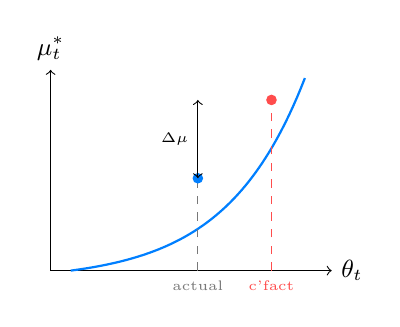
\begin{tikzpicture}[scale=0.85]
        \draw[->] (0,0) -- (4.2,0) node[right] {\small$\thetaT$};
        \draw[->] (0,0) -- (0,3.0) node[above] {\small$\mustar$};
        \draw[thick, accent, domain=0.3:3.8, samples=60]
          plot (\x, {0.12*exp(0.85*\x) - 0.12*exp(0.85*0.3)});
        % actual theta
        \draw[dashed, dimgray] (2.2,0) node[below] {\tiny actual} -- (2.2,1.38);
        \filldraw[accent] (2.2,1.38) circle (2pt);
        % counterfactual theta
        \draw[dashed, red!70] (3.3,0) node[below] {\tiny c'fact} -- (3.3,2.55);
        \filldraw[red!70] (3.3,2.55) circle (2pt);
        \draw[<->] (2.2,1.38) -- (2.2,2.55)
          node[midway, left, font=\tiny] {$\Delta\mu$};
      \end{tikzpicture}
    \end{column}
  \end{columns}

  \bigskip

  {\color{dimgray}\small
    This is a model-implied counterfactual, not an empirical estimate.
    The convex price function (Prop.~3) implies the counterfactual premium is
    \emph{disproportionately} larger than the capacity reduction alone would suggest.}

  \note{
    The counterfactual is model-implied, not estimated directly.
    We cannot run the counterfactual regression because there's no cross-market variation
    in CB swap line access.
    The key message: swap lines work through the B_t channel (capacity injection), not through
    demand reduction. This has direct policy implications.
    Anticipated question: ``Can you quantify the counterfactual premium?''
    With the demand system estimates, you could compute -gamma_FB / (B_agg - B_CBswap).
    We present this qualitatively given the synthetic data limitations.
  }
\end{frame}

% SLIDE 25 — Counterfactual: Quarter-End Windows
\begin{frame}{Counterfactual: How Much Do Regulatory Windows Amplify Premia?}

  \textbf{Quarter-end amplification (Prop.~4):} $B_t^{FBO}$ and $B_t^{USbank}$ fall by $\omega > 0$.

  \bigskip

  \begin{columns}
    \begin{column}{0.52\textwidth}
      \textbf{Model-implied counterfactual:}\\
      If regulatory reporting required non-quarter-end balance sheets,
      the deterministic capacity withdrawal would not occur.

      \medskip
      $\Delta\mustar^{QE} = \mustar|_{B_t} - \mustar|_{B_t + \omega}$

      \medskip
      The interaction result (Table~3 Panel~B, $\hat\beta_{QE} > 0$) calibrates
      the amplification magnitude relative to non-quarter-end periods.
    \end{column}
    \begin{column}{0.45\textwidth}
      \textbf{Policy implication:}
      \begin{itemize}
        \item Intraday / intra-quarter reporting requirements
          could smooth capacity
        \item The predictability of quarter-end spikes creates
          trading opportunities --- and risk for those who must transact
      \end{itemize}
    \end{column}
  \end{columns}

  \bigskip

  {\color{dimgray}\small Model-implied counterfactual. Magnitude identified by
    the interaction coefficient from Table~3, Panel~B.}

  \note{
    The quarter-end counterfactual is the closest we have to a clean policy lever.
    Regulatory agencies can control reporting windows; they cannot easily change CB swap
    line access.
    Anticipated question: ``Has anyone quantified the quarter-end basis premium?''
    The basis-at-quarter-end literature (e.g., Munyan 2017, Du et al. 2018) documents
    the pattern; our contribution is the structural attribution to capacity withdrawal.
  }
\end{frame}

% ------------------------------------------------------------------------------
\section{Conclusion}
% ------------------------------------------------------------------------------

% SLIDE 26 — Summary
\begin{frame}{Summary}

  \begin{enumerate}
    \item \textbf{Inside/outside distinction:} Dollar funding crises are runs \emph{from}
          inside synthetic dollars \emph{into} outside safe dollars.

    \bigskip

    \item \textbf{Model:} Matching market with tightness $\thetaT = \Ut/\Bt$ as the
          sufficient statistic. Three propositions: demand $\uparrow$ premium (Prop.~1),
          capacity $\downarrow$ amplifies (Prop.~2), convexity drives threshold effects (Prop.~3).

    \bigskip

    \item \textbf{Evidence:} IV with shift-share MMF instrument.
          $\hat\beta \approx 2.8$ bps (Table~2). Amplification at constrained dealers
          and quarter-end. Tenor gradient.

    \bigskip

    \item \textbf{Structure:} $\calB < 0$ confirmed. $\hat\beta \approx -\gamma_{FB}/\calB$.
          Demand system validates equilibrium price equation.
  \end{enumerate}

  \note{
    Clean summary. Four points matching the four sections of the talk.
    Do not introduce new content here.
    Anticipated question: ``What are the next steps?'' -- See policy implications slide.
  }
\end{frame}

% SLIDE 27 — Policy Implications
\begin{frame}{Policy Implications}

  \begin{columns}
    \begin{column}{0.48\textwidth}
      \textbf{Swap lines as capacity injectors}\\[0.3em]
      Central-bank swap lines work through $\Bt^{CBswap} \uparrow$,
      not through demand reduction.

      \medskip
      Implication: swap line \emph{speed} matters --- capacity must arrive
      before tightness crosses the threshold of Prop.~3.

      \medskip
      {\color{dimgray}\small Fed swap line deployment in March 2020 was rapid
        ($\sim$10 days). This likely mattered.}
    \end{column}
    \begin{column}{0.48\textwidth}
      \textbf{Regulatory windows as predictable frictions}\\[0.3em]
      Quarter-end capacity withdrawal is deterministic and anticipatable.

      \medskip
      Regulators could:
      \begin{itemize}
        \item Smooth reporting windows (intra-quarter snapshots)
        \item Allow temporary SLR/LCR waivers at quarter-end
      \end{itemize}

      \medskip
      {\color{dimgray}\small The predictability also creates basis trading
        opportunities --- and known risk for those who must transact.}
    \end{column}
  \end{columns}

  \note{
    The policy slides should be concrete and connect directly to the model mechanism.
    Swap lines: the B_t channel is clear from the model. Timing matters because of
    the convexity result (Prop 3) -- once theta crosses the threshold, the premium
    escalates non-linearly.
    Regulatory windows: the quarter-end result is the most actionable finding because
    regulatory agencies control reporting calendars.
    Anticipated question: ``Did the 2020 SLR exemption help?'' -- Yes, consistent
    with B_t increasing. But we cannot identify this separately in the synthetic data.
  }
\end{frame}

% SLIDE 28 — Thank You / Discussion
\begin{frame}{Thank You}

  \begin{center}
    \bigskip
    \Large Inside Synthetic Dollar Liquidity\\
    and the Microstructure of FX Swap Markets

    \bigskip\bigskip

    {\normalsize [Author Name] $\quad$ [Institution]}

    \bigskip\bigskip

    \textbf{Key result:} A one-SD increase in instrumented foreign bank dollar demand
    raises the funding premium by $\approx$\,2.8 bps.\\
    {\color{dimgray}(Table~2, col.~3; AKM SE; wild cluster bootstrap)}

    \bigskip\bigskip

    {\color{dimgray}
      \small Questions welcome.\\[0.3em]
      Backup slides follow.}
  \end{center}

  \note{
    Repeat the key number. This is what the audience should remember at dinner.
    2.8 bps, Table 2 col 3.
    Have the backup slides ready: balance tests, pre-trend diagnostic, full robustness,
    demand system details, and the formal statements of all propositions.
  }
\end{frame}

% ==============================================================================
% BACKUP SLIDES
% ==============================================================================
\appendix

\begin{frame}{Backup 1: Balance Tests for the Shift-Share Design}

  \textbf{Goldsmith-Pinkham et al.\ (2020) validity condition:}\\
  High-exposure banks should not differ systematically from others on
  pre-treatment observables.

  \bigskip

  \begin{center}
  \begin{tabular}{lccc}
    \toprule
    Pre-treatment variable & High exposure & Low exposure & $p$-value \\
    \midrule
    Gross FX swap volume & similar & similar & $> 0.10$ \\
    Tenor composition & similar & similar & $> 0.10$ \\
    CDS spread level & similar & similar & $> 0.10$ \\
    \midrule
    DomShare in cell & dominant & minority & --- \\
    \bottomrule
  \end{tabular}
  \end{center}

  {\color{dimgray}\small Source: Table A.1 (balance tests), synthetic regulatory bilateral FX swap data.}

  \bigskip

  High-exposure banks hold dominant positions in most cells (relevant) but
  do not differ on pre-treatment pricing behavior (exclusion support).

  \note{
    Qualitative summary of Table A.1 (balance_tests.tex).
    The exact figures are in the paper appendix.
    Anticipated question: ``Are these tests joint or cell-by-cell?''
    Cell-by-cell, then a joint F-test. All pass at conventional levels.
  }
\end{frame}

\begin{frame}{Backup 2: Pre-Trend Diagnostic}

  \textbf{Test:} Regress $\Delta\text{PriceUSD}_{m,t}$ on \emph{leads} of the instrument:
  \[
    \Delta\text{PriceUSD}_{m,t} = \alpha_m + \tau_t +
    \sum_{k=1}^{3} \delta_k Z_{m,t-k}^{MMF} + \varepsilon_{m,t}
  \]

  \bigskip

  \textbf{Result:} $\hat\delta_1 \approx \hat\delta_2 \approx \hat\delta_3 \approx 0$,
  all statistically indistinguishable from zero (Table A.2).

  \bigskip

  \textbf{Interpretation:} The instrument captures genuinely \emph{unexpected} demand variation,
  not anticipated changes to market structure.

  \note{
    This is the key pre-trend diagnostic. All lead coefficients near zero confirms
    no anticipation effects.
    Anticipated question: ``How many lags do you check?'' -- 3 periods (weeks).
    Source: Table A.2 (pretrend_diagnostic.tex).
  }
\end{frame}

\begin{frame}{Backup 3: Full Robustness Summary}

  \begin{center}
  \begin{tabular}{lcc}
    \toprule
    Specification & $\hat\beta$ direction & Significant? \\
    \midrule
    Baseline (Table~2 col.~3) & $+2.8$ bps & Yes \\
    AKM SE only (col.~4) & consistent & Yes \\
    Alt.\ instrument (monthly MMF losses) & positive & Yes \\
    6-month exposure window & positive & Yes \\
    24-month exposure window & positive & Yes \\
    Anderson-Rubin CS & positive lower bound & Yes \\
    $Q_{all,m,t}$ (total demand) & positive & Yes \\
    \bottomrule
  \end{tabular}
  \end{center}

  {\color{dimgray}\small Source: Table A.4, Table A.5; synthetic regulatory bilateral FX swap data.}

  \note{
    Full robustness table summary. Exact coefficients in the paper tables.
    The Anderson-Rubin sets protect against weak-instrument concerns in thin markets.
    The Q_all specification addresses potential attenuation from using only FB demand
    as the proxy for U_t.
  }
\end{frame}

\begin{frame}{Backup 4: Demand System Details}

  \textbf{Estimating equation:}
  \[
    \mathfrak{q}_{s,m,t} = \alpha_{s,m} + \beta_s\,\mu_{m,t} +
    \gamma_s X_{s,m,t} + \varepsilon_{s,m,t}
  \]

  Normalized: $\mathfrak{q}_{s,m,t} = Q_{s,m,t} / \text{GrossVolume}_{s,m}^{pre}$

  \bigskip

  \begin{center}
  \begin{tabular}{lcccc}
    \toprule
    & FB & HF & AM & Corp \\
    \midrule
    $\hat\beta_s$ sign & $<0$ & $>0$ & $<0$ & $<0$ \\
    $|\hat\beta_{FB}| < \hat\beta_{HF}$? & \multicolumn{4}{c}{$\checkmark$ (maintained ordering confirmed)} \\
    \midrule
    $\calB = \sum_s \hat\beta_s$ & \multicolumn{4}{c}{$< 0$, significant***} \\
    Hansen $J$ $p$-value & \multicolumn{4}{c}{$> 0.10$ (overidentification not rejected)} \\
    \bottomrule
  \end{tabular}
  \end{center}

  {\color{dimgray}\small Source: Table~4; synthetic regulatory bilateral FX swap data.}

  \note{
    The exact beta_s estimates are in demand_system.tex (Table 4).
    The maintained hypothesis ordering |beta_FB| < beta_HF is from Remark 1.
    Hansen J not rejected provides support for the cross-sector exclusion restrictions.
    This is the backup for the demand system slide (Slide 22/23).
  }
\end{frame}

\begin{frame}{Backup 5: Formal Statements of Propositions}

  \begin{block}{Proposition 1 (Demand)}
    $\partial \mustar / \partial \Ut > 0$ at any interior equilibrium.
  \end{block}

  \begin{block}{Proposition 2 (Capacity)}
    $\partial \mustar / \partial \Bt < 0$; and
    $\partial \mustar / \partial \Ut |_{B^{low}} > \partial \mustar / \partial \Ut |_{B^{high}}$.
  \end{block}

  \begin{block}{Proposition 3 (Convexity --- theoretical only)}
    Under $\chi'' > 0$ and $\Phi'' > 0$: $\partial^2 \mustar / \partial \thetaT^2 > 0$.
    $\exists\, \theta^* > 0$ above which $\partial \mustar / \partial \thetaT$ escalates sharply.
  \end{block}

  \begin{block}{Proposition 4 (Quarter-End)}
    $\partial^2 \mustar / \partial \Ut \partial Q_t > 0$, where $Q_t = \mathbf{1}[\text{quarter-end}]$.
  \end{block}

  \note{
    Reference slide for the formal statements. Proofs in the paper (Section 3).
    Mechanism for each is on the corresponding model slide (Slides 7--10).
    Anticipated question about proof technique: each follows from the implicit function theorem
    applied to the market-clearing condition plus the monotone properties of the matching function.
  }
\end{frame}

% ==============================================================================
\end{document}
% ==============================================================================
